\section{Implementation}
\label{sec:implementation}

This section presents the architecture of the implementation of our approach first. After that, we introduce the algorithm for validating the traceability links, and for code selection completion which helps the user to complete the code piece selection when part of a syntax element is selected.

\subsection{Architecture}

\begin{figure}
\begin{center}
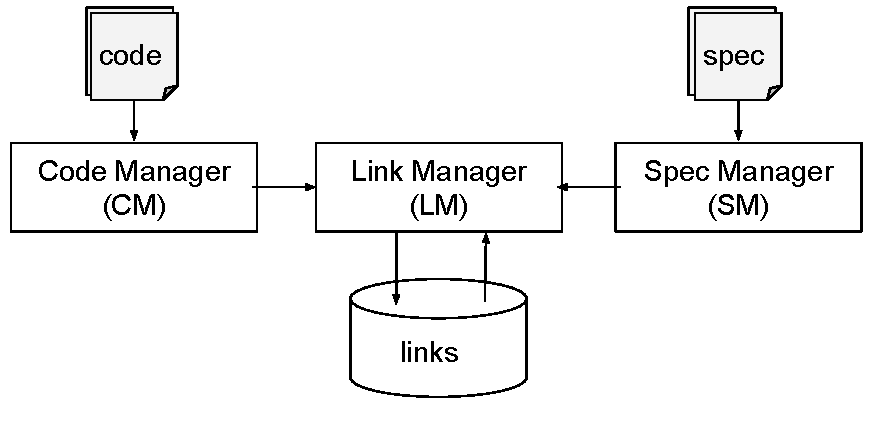
\includegraphics[width=0.55\textwidth]{architecture}
\caption{coDoc Architecture and Features}
\label{fig:architecture}
\end{center}
\end{figure}

The architecture of our approach is shown in Figure \ref{fig:architecture}. 
There are three types of data here, 1) code, 2) spec, and 3) traceability links.
These data are consumed by three components: code manager (CM), spec manager (SM) and link manager (LM).
\begin{enumerate}
\item \textit{Link Manager.} Traceability link manager get the highlighted code piece from code manager and the highlighted spec piece from spec manager, and create traceability link for these two piece of information. It also reads the traceability link data, verify the validity of the link,
and highlights the code and document pieces that are related.
\item \textit{Code Manager.} Code manager reuses C/C++ Development Tool (CDT) editor from Elipse\footnote{\texttt{\url{http://www.eclipse.org}}} to parses the code, 
and highlights syntax elements. It can highlight the piece of code based on the information provided by the user or the link manager.
\item \textit{Spec Manager.} Spec manager renders the pdf content, can support select and highlight spec content, and communicate with the link manager.
\end{enumerate}

We implemented coDoc as an Elipse Rich Client Program (RCP), 
which can make our tool share the appearence in Eclipse that is familiar by many programmer.
Figure \ref{fig:platformview} is the screenshot of the tool.
The bottom is the UI for link manager, while the top left part and top right side are the UI for code manager and spec manager repectively.

% convert platformview.png platformview.eps
\begin{figure}
\begin{center}
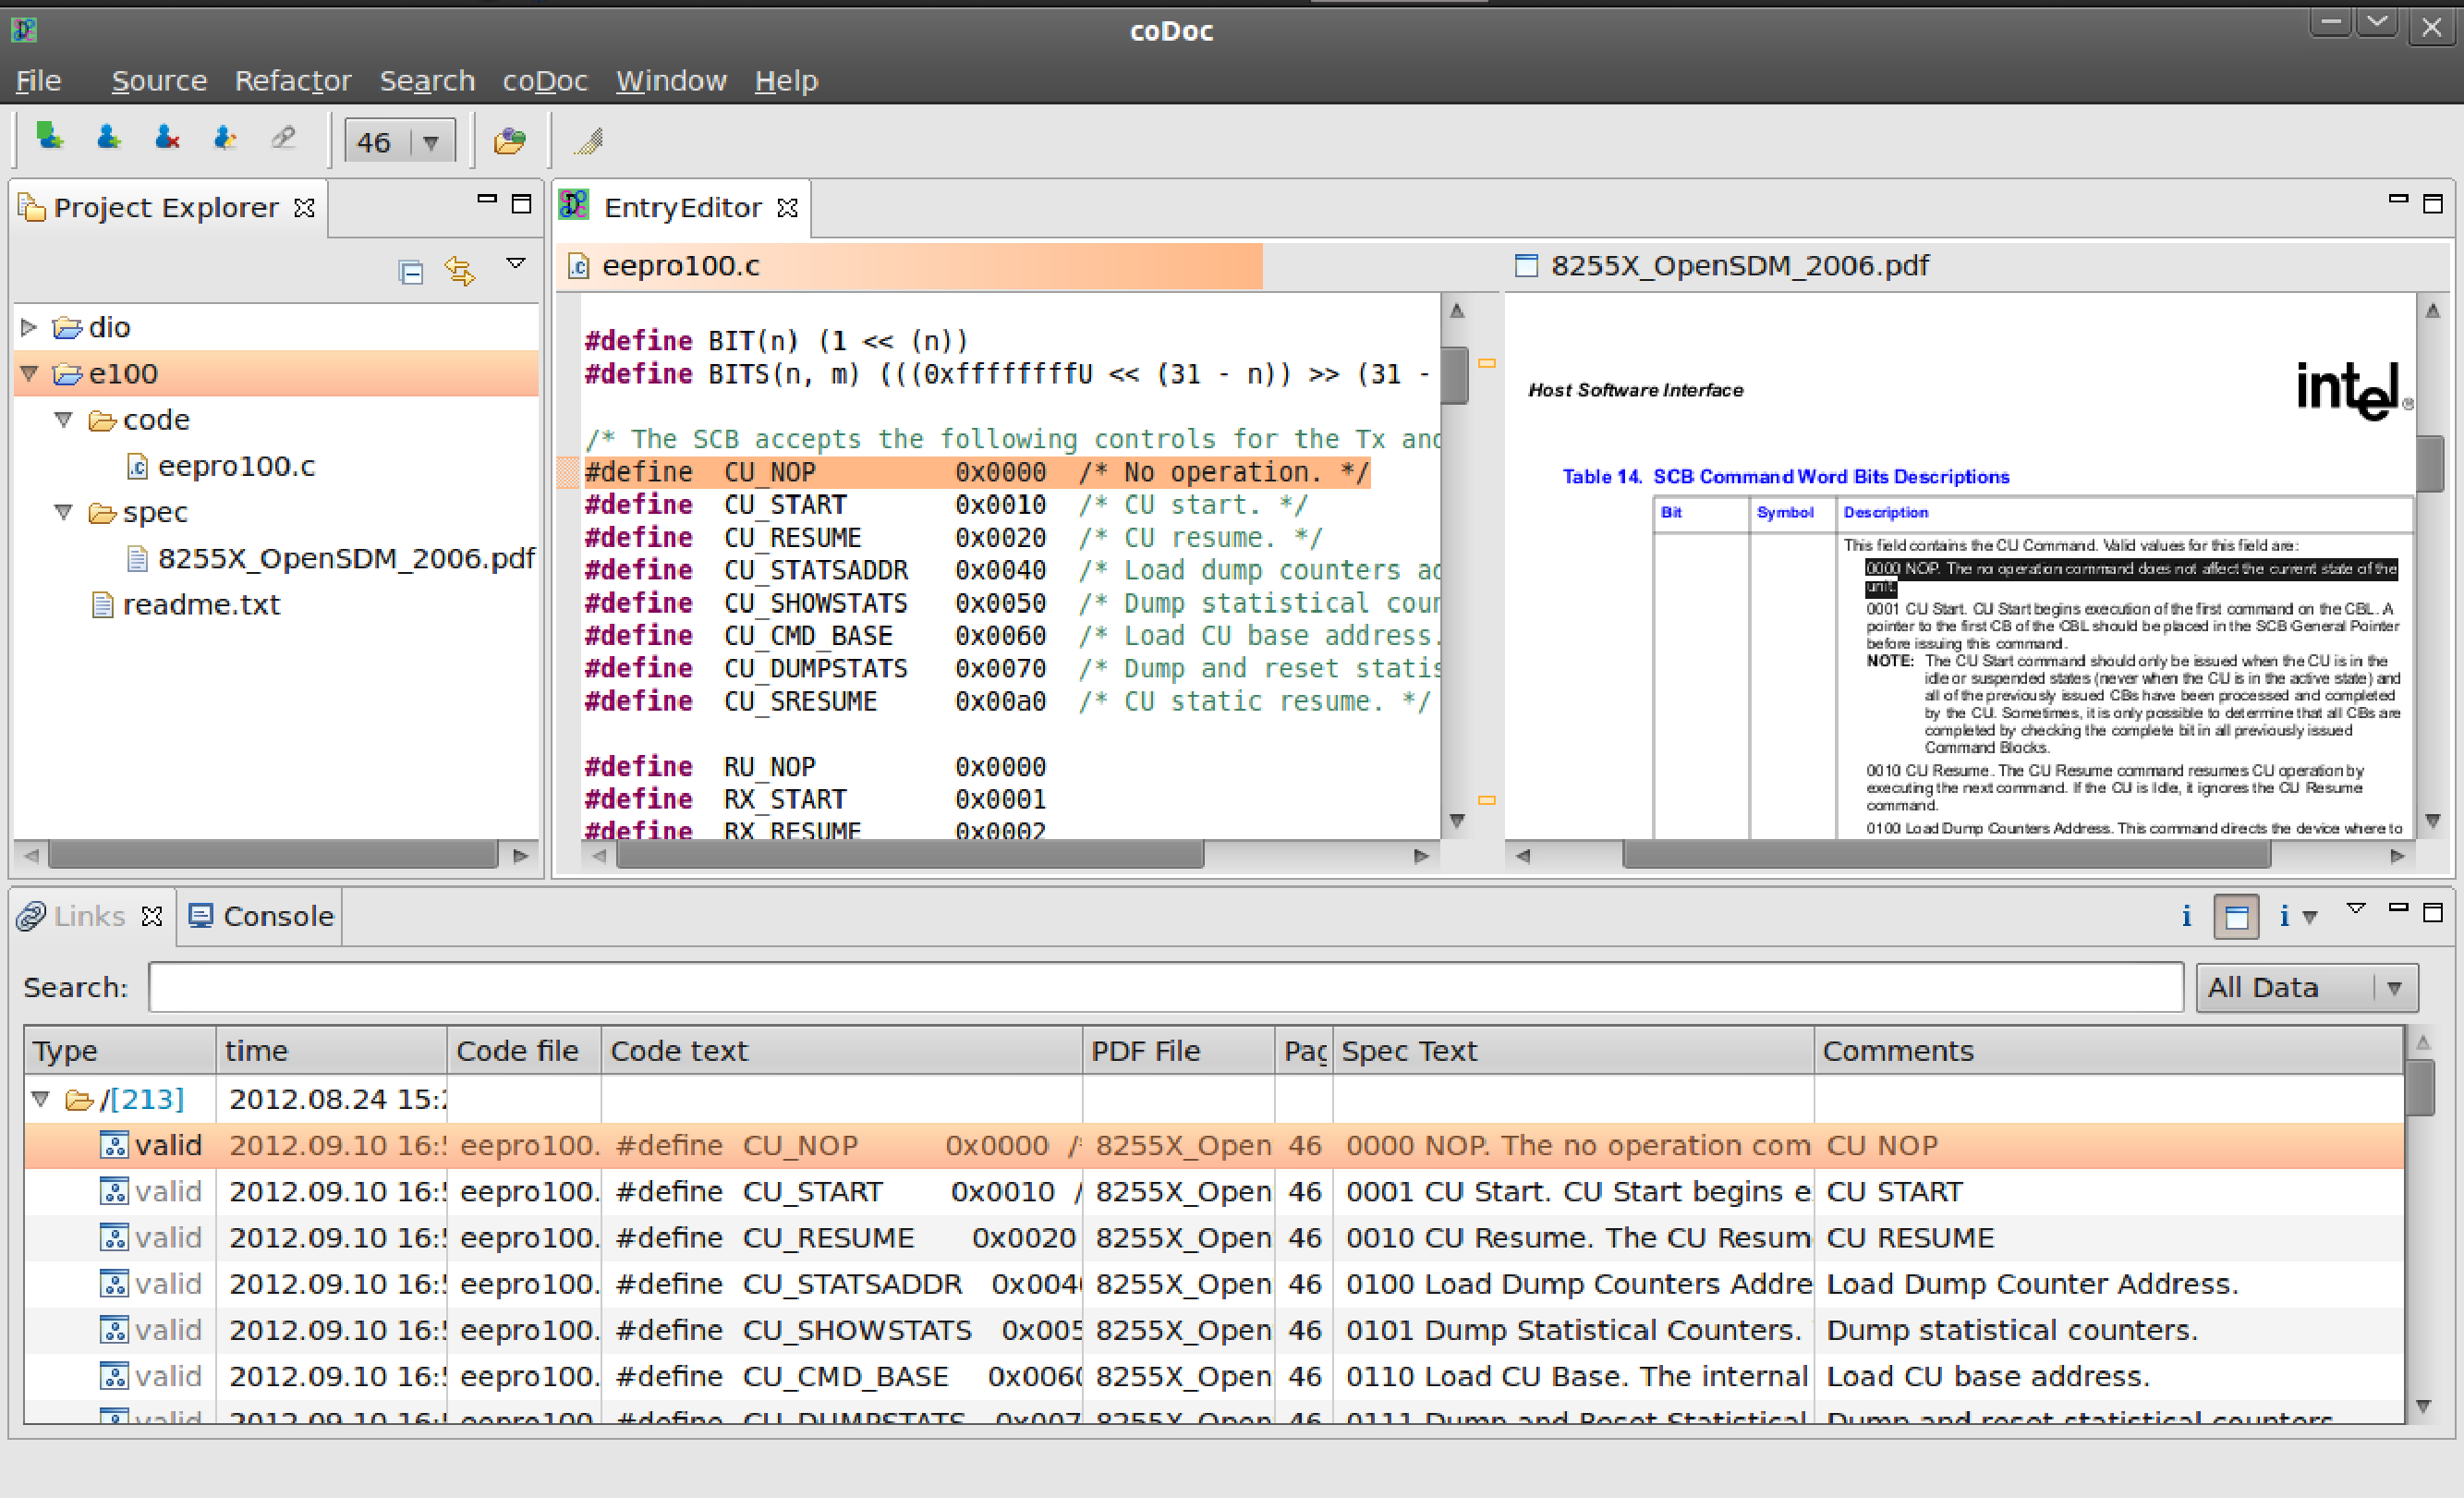
\includegraphics[width=\textwidth]{platformview}
\caption{coDoc Platform View}
\label{fig:platformview}
\end{center}
\end{figure}


\subsection{Link Validation}

\begin{algorithm}[!h]
\DontPrintSemicolon
\SetKwComment{tcp}{\hfill$\triangleright$ }{}
\SetCommentSty{emph}
$AST \leftarrow \textsc{Gen-AST}(code)$\;
$\langle RES, CONTENT_C \rangle \leftarrow \textsc{Get-Code-Content}(AST, link.code.path)$\;
\If{$RES = FAIL$} {
\Return $FAIL$\;
}
$RES \leftarrow \textsc{Compare-Content}(CONTENT_C, link.code.content)$\;
\If{$RES = FAIL$} {
\Return $FAIL$\;
}
$CONTENT_S \leftarrow \textsc{Get-Spec-Content}(spec, link.spec.path)$\;
$RES \leftarrow \textsc{Compare-Content}(CONTENT_S, link.spec.content)$\;
\If{$RES = FAIL$} {
\Return $FAIL$\;
}
\Return $SUCCESS$\;
\caption{$\textsc{Traceability-Link-Validation}(link)$}
\label{alg:validate}
\end{algorithm}

%\begin{figure}[h!]
%  \begin{center}
%    \begin{minipage}[b]{0.6\linewidth}
%      \centering
%      \renewcommand{\ttdefault}{pcr}
%      \begin{lstlisting}
%for each leaf node in syntax tree
%  for each node in anchor
%    node string compare
%\end{lstlisting}
%\end{minipage}
%\caption{Pseudocode for Link Validation}
%\label{fig:validate}
%\end{center}
%\end{figure}

When code evolves, we need to validate the existing traceability links.
Once an invalid traceability links is found, we should report it to let user correct it manually.
To check the validity of the traceability links, we record the content of the code piece and the spec piece when generating the links.
The content is used later to compare with the content to which the path points to when code changes.
The validation process basically go through each traceability link in the database, 
and check whether the link is valid or not.
Algorithm~\ref{alg:validate} presents the pseudo-code for check the validation of one single traceability link.
Line 1 - line 7 check the validity of the code piece part of the traceability link.
Line 1 generates the AST for the current code first.
Line 2 then invokes the function \textsc{Get-Code-Content} with the path of the code piece as input, identify the code piece in the new AST, and return the content of the code piece if the code piece is identified successfully.
If the path of the code piece cannot identify any code piece or can identify more than one code piece, the function \textsc{Get-Code-Content} reports failure.
Line 5 compare the the new content extracted from the new code with the recorded old content, and fail if the two contents do not match.
After finishing check the code piece part, line 8 - line 11 of the algorithm check the spec piece part in a similar flow.
If no failure happens, the algorithm return successfully at line 12.


\subsection{Code Selection Completion}

\begin{algorithm}[!h]
\DontPrintSemicolon
\SetKwComment{tcp}{\hfill$\triangleright$ }{}
\SetCommentSty{emph}
$AST \leftarrow \textsc{Gen-AST}(code)$\;
$SEQUENCE_{LEAF} \leftarrow \textsc{Gen-Leaf-Sequence}(AST)$\;
$POC_{AST} \leftarrow \textsc{To-AST-Based}(SEQUENCE_{LEAF}, selection_{org})$\;
$selection_{new} \leftarrow \textsc{To-Offset-Based}(POC_{AST})$\;
\Return $selection_{new}$\;
\caption{$\textsc{Complete-Code-Selection}(selection_{org})$}
\label{alg:completion}
\end{algorithm}

To improve the user experience of coDoc, we help users to select the code pieces when creating traceability links.
Our approach is based on the fact that it is usually meaningless to have part of the basic code elements as the code piece of the traceability links.
For example, we do not create a link between half of the variable and the spec piece.
We assume that every selected piece of code is composed of valid syntax elements.
Based on this assumption, we can help the user to automatically complete their selection when they only select part of the syntax element, like a variable, a constant, and etc. 
Algorithm \ref{alg:completion} outlines our approach.
This algorithm takes a code selection in offset based format,
and returns a new code selection in offset based format.
We choose offset based format because Eclipse use this format to highlight the code piece.
The algorithm basically includes two parts: (1) line 1 - line 3 force the input selection to be aligned by transforming it from offset based code piece to AST based code piece. (2) line 4 generates the required format by transforming AST based code piece back to offset based code piece.
As we discussed before, AST based representatioin is a sequence of AST leaf nodes in DFS visit order, which is the same order as in the source code.
The AST based code piece covers all the meaningful part of the original offset based code piece.
To transform the offset based code piece to AST based code piece, 
we get the sequence of leaf nodes of AST in line 1 and line 2,
and then match the leaf node sequence with the code piece to get the AST based representation.
The leaf node in the AST based representation is determined this way: if the leaf node contains any part of the selected code, then the leaf node is in the representation.
After we get the AST based representation,
we transform it back to offset based reprensentation, and return it.
This way, each time the user make a selection,
our engine adjust the selection to valid syntax boundary.

